% !TEX root = mainthesis.tex
%Chapter 8

\renewcommand{\thechapter}{8}

\chapter{Unconventional topology with a Rashba SOC quantum gas}
\label{ch:Rashba}

As I mentioned in the previous Chapter topological order is present in a wide range of physical systems and is quantified by integer valued topological invariants such as the Chern number. In this Chapter I describe the experiments to engineer and characterize the topology of a quantum gas with Rashba-type SOC. Our system broke from the conventional mold of topological materials and I show that its resulting topological indices can take both integer and half-integer values. If the concept of half-integer invariants does not sound odd to you should think of a donut with half a hole. 

Ultracold atomic systems are an emerging platform for engineering topological lattices, from the Harper-Hofsdater model\cite{miyake_realizing_2013,aidelsburger_realization_2013}, the Haldane model\cite{jotzu_experimental_2014}, to the Rice-Mele model\cite{lu_geometrical_2016,lohse_thouless_2016} as well as assembling spin-orbit coupled lattices without analogues in existing materials\cite{wu_realization_2016,sun_highly_2018}. 

Experimental realizations of topological materials have mostly focused on engineering different topological bands (with different Berry curvatures) in lattice systems, where the BZ is always a torus. Here I show that by eliminating the lattice potential and thereby changing the BZ from ${\mathbb T}^2$ to ${\mathbb R}^2$, i.e. from a torus to a Cartesian plane, it is possible to create topological branches of the dispersion relation with half-integer Chern number. In our experiments we created both topological and non-topological dispersion branches by introducing Rashba-like SOC\cite{campbell_realistic_2011, huang_experimental_2016, meng_experimental_2016} to a cold quantum gas. %In contrast to crystalline materials, where topological indices take on integer values, our continuum system reveals an unconventional half-integer Chern number, potentially implying new forms of topological transport.

This Chapter is organized in the following way: First I will give a general overview of Rashba SOC and will describe theoretical proposals for engineering this type of coupling in ultracold atom systems. Then I will describe our experimental implementation of Rashba SOC in the lab using a trio of Raman coupled CDD states (Chapter~\ref{ch:clock_states}) and validate our quantum engineering using Fourier transform spectroscopy (Chapter~\ref{ch:Fourier_spectroscopy}). Finally I will describe a quantum state tomography procedure to measure the eigenstates of our system, and directly obtain the Chern number. 

To avoid confusion between dressed state $xyz$ labels and Cartesian coordinates, in this Chapter I will use the numbers $1,2,3$ to label the coordinates $\ex, \ey, \ez$ and the letters $x,y,z$ to label dressed state parameters. 

\section{Rashba spin-orbit coupling}

Rashba SOC~\cite{bychkov_oscillatory_1984} appears in condensed matter systems where electrons are confined in a 2D plane and experience an intrinsic out-of-plane electric field. If the electron's momentum is given by $\hbar\k=\hbar(k_x\ex+k_y\ey)$ and the electric field is $\mathbf{E}=E\ez$, in the electron's moving frame there will be a momentum dependent magnetic field $\mathbf{B}_{\rm SOC}=-\hbar\k/m\times\mathbf{E}/c^2=\hbar E/mc^2(-k_y, k_x, 0)$. The interaction between the electron's spin with this field through the magnetic Zeeman interaction $-\mathbf{\mu}\cdot{\mathbf{B}_{\rm SOC}}$ gives rise to the SOC Hamiltonian
%
\begin{equation}
	\hat{H}_{\rm SOC}=\frac{2\alpha}{m}(k_y\hat{\sigma}_x-k_x\hat{\sigma}_y)
	\label{eq:Rashba_ham}
\end{equation}
%
where $\alpha=g\mu_BE/c^2$, $g$ is the electrons gyromagnetic ratio, $\mu_B$ is the Bohr magneton and $\hat{\sigma}_i$ are the Pauli matrices. 

The Rashba dispersion relation is characterized by having a Dirac point located at $\k=0$ (see Chapter~\ref{sec:2_level_topology}) and a degenerate ground state that is described by the ring $k_x^2+k_y^2=\alpha^2$. \note{TODO: Make figure} If we combine Equation~\ref{eq:Rashba_ham} with the free particle Hamiltonian the Hamiltonian can can be written as $\hat{H}=(\hbar\k-\hat{\mathbf{A}})^2/2m$ where $\mathbf{\hat{A}}=\alpha(\hat{\sigma}_y\ex-\hat{\sigma}_x\ey)$ can be interpreted as a (matrix valued) non-abelian gauge potential whose elements do not commute. This term is closely related to the Berry connection discussed in Chapter~\ref{sec:Berry phase and curvature}. This in combination with the presence of the Dirac point hints to us that a system with Rashba SOC has non-trivial topology. 

SOC is also a necessary ingredient for realizing $\mathds{Z}_2$ topological insulators and the quantum spin-Hall effect. Furthermore, the degeneracy of the ground state single particle eigenstates could open the possibility of studying strongly correlated phases in the presence of interactions for systems of both fermions and bosons~\cite{stanescu_spin-orbit_2008,sedrakyan_composite_2012,hu_probing_2011}. SOC systems offer the possibility of studying a wide range of interesting physics and naturally using ultracold atomic systems to engineer SOC, and in particular Rashba type SOC, has been a longstanding goal~\cite{galitski_spin-orbit_2013}. 


\section{Rashba SOC for neutral atoms}
\label{sec:rashba_ring_coupling}

Proposals for engineering Rashba type SOC in neutral atoms consist in using lasers to link internal states of an atom with its linear momentum. In order to achieve non-trivial gauge potentials it is necessary to couple $N\geq3$ levels (see~\cite{goldman_light-induced_2014}). I will describe the proposal by~\cite{campbell_realistic_2011} which considers a `ring coupling' which is shown in Figure~\ref{fig:rashba_ring_coupling} for the case of $N=3$. The states $\ket{j}$ represent internal atomic states and they are linked to each other with complex valued matrix elements $\frac{\Omega_j}{2}e^{i\k_{j}\cdot\x}$, where $\k_{j}$ is a momentum transfer associated with the $\ket{j}\rightarrow\ket{j+1}$ transition and $\Omega_i=e^{i\phi_i}\vert\Omega\vert$ represents the coupling strength. We require that $\sum\k_i=0$ so that no momentum is transfered when a closed loop $\ket{1}\rightarrow\ket{2}\dots \rightarrow\ket{N}\rightarrow\ket{1}$ is completed. For this case the $\k_i$ momenta vectors can be written as $\k_j=\mathbf{K}_{j+1}-\mathbf{K}_j$, and we make $\mathbf{K}_j=\kl\sin(2\pi j/N)\ex+\kl\cos(2\pi j /N)\ey$, corresponding to the vertices of an N sided regular polygon. We can further make a gauge transformation such that we can replace the phases $\phi_i$ associated to each coupling with $\bar{\phi}=\sum_i\phi_i/N$.

\begin{figure*}[htb]
\begin{center}
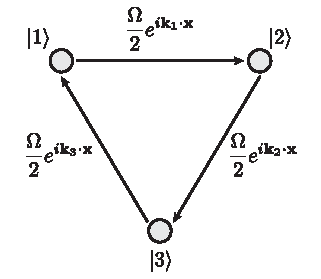
\includegraphics[]{Figures/Chapter8/Rashba_ring_coupling.pdf}
\caption[The Rashba ring coupling]{The Rashba ring coupling. To generate Rashba SOC in a system of cold atoms it is necessary to cyclically couple $N\geq3$ internal states such that the transition $\ket{j}\rightarrow\ket{j+}1$ has a momentum transfer $\k_j$ and $\sum_j\k_j=0$ such that there is no momentum transfer for a closed loop $\ket{1}\rightarrow\ket{2}\dots\ket{N}\rightarrow\ket{1}$. The ring coupling combined with the free particle Hamiltonian give rise to a 2-level subspace that can be described to first order by the Rashba Hamiltonian}
%
\label{fig:rashba_ring_coupling}
\end{center}
\end{figure*}
%
The Hamiltonian describing this coupling along with the kinetic term is 
%
\begin{equation}
	H_{j, j'}=\frac{\hbar^2 k^2}{2m}\delta_{j,j'} + \frac{\Omega}{2}(e^{i(\bar{\phi}+\k_j\cdot\x)}\delta_{j, j'+ 1} + {\rm h.c.}),
\end{equation}
%
and after applying the unitary transformation $U_{j, j'}=\exp[i\mathbf{K}_i\cdot\x]\delta_{j,j'}$\footnote{This transformation is equivalent to applying a state dependent momentum boost $\k\rightarrow \k +\mathbf{K}_j $} it gets transformed to 
%
\begin{equation}
	H_{j,j'}=\frac{\hbar^2}{2m}\vert \q +\mathbf{K}_j\vert^2\delta_{j,j'} + \frac{\Omega}{2}(e^{i\bar{\phi}}\delta_{j, j'+ 1} + {\rm h.c.}),
	\label{eq:rashba_tight_binding}
\end{equation}
%
where I have replaced the momentum $\k$ by the quasimomentum $\q$. The off diagonal terms of Equation~\ref{eq:rashba_tight_binding} can be related to a 1D periodic tight-binding Hamiltonian with hopping elements $\Omega/2$ where the internal states $\ket{j}$ represent lattice sites and completing one loop corresponds to gaining a `flux' of $N\bar{\phi}$. It is helpful to write the Hamiltonian in a basis that is conjugate to the index $j$
%
\begin{equation}
	\ket{l}=\frac{1}{\sqrt{N}}\sum_{j=1}^N e^{i2\pi jl/N}\ket{j}
\end{equation}
%
where the index $l$ is analogous to the crystal momentum index for a Bloch Hamiltonian. In this new basis, terms with oscillatory components (e.g. $\vert \q + \mathbf{K}_j\vert$) in the diagonals are displaced to the off-diagonal and oscillatory terms in the off diagonal are displaced to the diagonal. Under this basis the Hamiltonian starts looking very much Rashba-like
%
\begin{equation}
	H_{l,l'} = \left[\frac{\hbar^2}{2m}(q^2+ k_L^2)+E_l\right]\delta_{l,l'} + \frac{\hbar^2\kl}{m}\left[(iq_x+q_y)\delta_{l-1,l'}+{\rm h.c}\right],
	\label{eq:ring_coupling_ft}
\end{equation}
%
where $E_L=2\hbar\Omega\cos(2\pi l/3+\bar{\phi})$ correspond to the eigenenergies when $q=0$. The phase $\bar{\phi}$ can be tuned such that a pair of states with consecutive $l$ index become degenerate, indicating the presence of a Dirac point at $q=0$. Figure~\ref{fig:ring_coupling_energies} shows the energies $E_l$ for $N=3$ and $\bar{\phi}=0$.

\begin{figure*}[htb]
\begin{center}
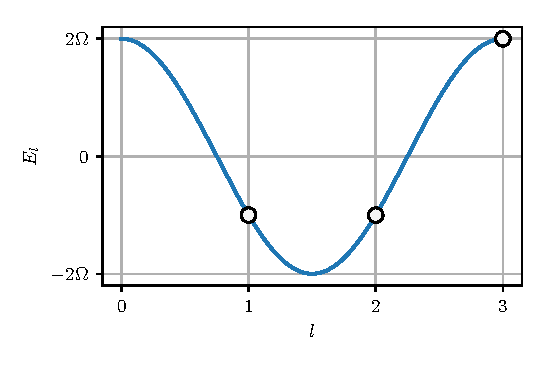
\includegraphics[]{Figures/Chapter8/ring_coupling_energies.pdf}
\caption[Rashba ring coupling eigenenergies]{Eigenenergies of Equation~\ref{eq:ring_coupling_ft} for $q=0$ for $N=3$ and $\bar{\phi}=0$. For this particular choice of phase, the energies of the $l=1$ and $l=2$ states become degenerate}
\label{fig:ring_coupling_energies}
\end{center}
\end{figure*}

We can consider the degenerate states corresponding to two consecutive $\ket{l}$ states as pseudospins which are described to zeroth order by the Rashba plus free particle Hamiltonian
%
\begin{equation}
	\hat{H}^{(0)} = \frac{\hbar^2q^2}{2m} + \frac{\hbar^2\kl}{m}(\hat{\sigma_x}q_y-\hat{\sigma}_yq_x), 
\end{equation}
 %
with spin orbit coupling strength given by $\alpha=\hbar^2k_L/2$. The zeroth-order Hamiltonian has continuous rotational symmetry while we the proposed ring coupling only has only discrete rotational symmetry. The symmetry of the Hamiltonian is recovered when higher order corrections of the Hamiltonian are included. The complete expressions for the higher order terms for $N=3$ and $N=4$ can be found in~\cite{campbell_realistic_2011}, and they are reminiscent of quadratic and cubic Dresselhaus SOC~\cite{stanescu_spin_2007}. The largest leading order term is inversely proportional to $\Omega^2$ so that this ring-coupling scheme results in a more `Rashba-like' Hamiltonian as one goes to higher coupling strengths. Figure~\ref{fig:rashba_alien} shows level curves of the ground state eigenenergies of Equation~\ref{eq:ring_coupling_ft} for $N=3$ and $\bar{\phi}=0$ for increasing $\Omega$. At low $\Omega$ the dispersion has discrete rotational symmetry and is characterized by three local minima. As $\Omega$ is increased the local minima start merging into each other and in the large $\Omega$ limit we recover the characteristic Rashba ring-like dispersion.   

\begin{figure*}[htb]
\begin{center}
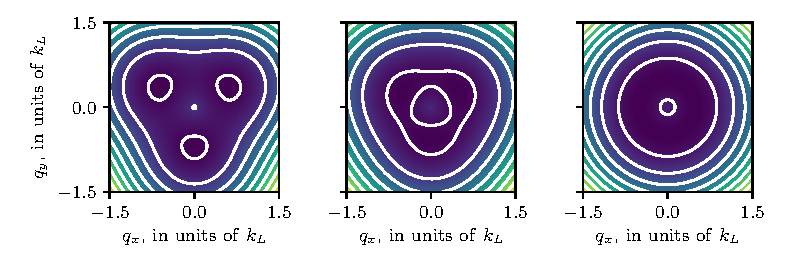
\includegraphics[]{Figures/Chapter8/rashba_alien.pdf}
\caption[Rashba ring coupling ground state dispersion]{Ground state dispersion relation of Equation~\ref{eq:ring_coupling_ft} for $N=3$ and $\bar{\phi}=0$ for $\Omega=\unit[1.75]{\El}$ (left), $\Omega=\unit[3.5]{\El}$ (middle) and $\Omega=\unit[175]{\El}$ (right). Higher order corrections to $\hat{H}^{(0)}$ decay as $1/\Omega^2$ and in the large $\Omega$ limit we recover the Rashba ring dispersion.}
\label{fig:rashba_alien}
\end{center}
\end{figure*}

% So far we have only considered the case where all the coupling strengths and the vectors $\k_j$ are symmetric. In the lab it might be hard due to constraints imposed by the capabilities of an experimental apparatus. As one departs from the ideal ring-coupling, we find that the resulting dispersion can looses its discrete rotational symmetry. While this perturbations can have a significant impact on the dispersion, the Dirac point is remarkably robust and as long as $\bar{\phi}$ is such that there are at least two degenerate states in the ideal ring coupling case the Dirac point will remain gapless although it might move from $\q=0$. The exact location of the Dirac point as a function of $\Omega_i$ and $\q$ for an imperfect ring-coupling scheme is derived in \cite{huang_experimental_2016}. Figure~\ref{fig:rashba_perturbed} shows some examples of how the ground state dispersion is modified when the vectors $\mathbf{K}_j$ that don't lie in the vertices of a regular polygon and when the amplitude of $\Omega$ is state dependent. 

% \begin{figure*}[htb]
% \begin{center}
% 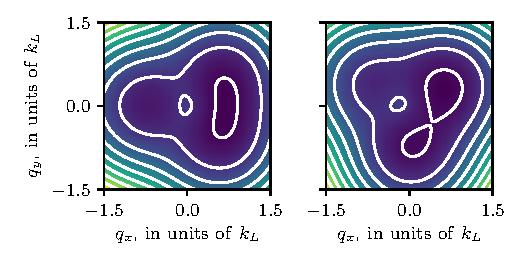
\includegraphics[]{Figures/Chapter8/rashba_perturbed.pdf}
% \caption[Perturbed Rashba dispersion]{(left) Ground state dispersion relation of Equation~\ref{eq:ring_coupling_ft} for $N=3$ and $\bar{\phi}=0$ for $\Omega=\unit[1.75]{\El}$ but $\mathbf{K}_j$ that don't correspond to to the vertices of an isosceles triangle rather than an equilateral triangle. Ground state dispersion for symmetric $\mathbf{K}_j$ but state dependent $\Omega=$. In both cases the discrete rotational symmetry is lost but the gapless Dirac point remains.}
% \label{fig:rashba_perturbed}
% \end{center}
% \end{figure*}

\section{Experimental implementation of Rashba SOC}

 We implemented the ring-coupling scheme and thereby engineered Rashba SOC by resonantly coupling three internal atomic states using two-photon Raman transitions\cite{campbell_rashba_2016} as depicted in Figure~\ref{fig:Schematic}. As shown in Figure~\ref{fig:Schematic}a, the engineered system consisted of an effective spin-1/2 Rashba subspace, along with a topologically trivial high-energy branch. Our engineered Rashba system had a single Dirac cone near $\q=0$, where the two lower dispersion branches become degenerate and the Berry curvature becomes singular. Each of these branches extend to infinite momentum, making the supporting manifold a plane rather than a torus. We characterized this system using both spectroscopy and quantum state tomography. This allowed us to measure the dispersion branches and directly observe the single Dirac point linking the lowest two branches as well as to reconstruct the Berry connection to derive the associated Chern numbers. \note{TODO:maybe the stuff of plane and torus doesn't go here}


%%%%%%%%%%%%%%%%%%%%%%%%%%%%%%%%%%%%%%%%%%%%%%%%%%%%%%%%%%%%%%%%%%
%
% Brief descrpiption of Rashba SOC: theory and implementation
%
%%%%%%%%%%%%%%%%%%%%%%%%%%%%%%%%%%%%%%%%%%%%%%%%%%%%%%%%%%%%%%%%%%

\begin{figure*}[htb]
\begin{center}
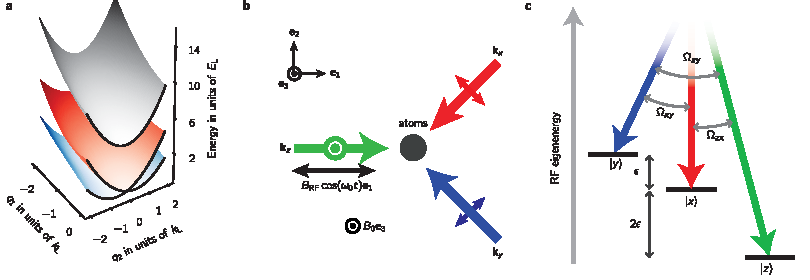
\includegraphics[width=\textwidth]{Figures/Chapter8/fig1.pdf}
\caption{{\bfseries a} Our engineered dispersion consisted of a two-level Rashba subspace (red and blue) with a single Dirac point linking the lowest two branches and a topologically trivial higher branch (gray). {\bfseries b} We generated $\xyz$ states by combining a bias magnetic field along $\mathbf{e}_3$ with an RF magnetic field oscillating along $\mathbf{e}_1$. These states were coupled by three cross-polarized Raman laser beams propagating along $\mathbf{e}_1$, $\mathbf{e}_2-\mathbf{e}_1$ and $-\mathbf{e}_1-\mathbf{e}_2$. {\bfseries c} Each pair of Raman lasers was in two-photon resonance with a single transition between the $\xyz$ states which we coupled strengths $(\Omega_{zx}, \Omega_{xy}, \Omega_{yz})/2\pi=\unit[(12.6(5), 8.7(8), 10(1))]{kHz}$.}
\label{fig:Schematic}
\end{center}
\end{figure*}

%%%%%%%%%%%%%%%%%%%%%%%%%%%%%%%%%%%%%%%%%%%%%%%%%%%%%%%%%%%%%%%%%%
%
% Brief details on experimental implementation
%
%%%%%%%%%%%%%%%%%%%%%%%%%%%%%%%%%%%%%%%%%%%%%%%%%%%%%%%%%%%%%%%%%%

All of our experiments started with about with $N\approx 1\times 10^6$$\Rb87$ atoms in a crossed optical dipole trap\cite{lin_rapid_2009}, with frequencies $(f_1,f_2,f_3) \approx \unit[(70, 85, 254)]{Hz}$, just above the transition temperature for Bose-Einstein condensation. We initially prepared the atoms in the $\ket{F=1, m_F=-1}$ state of the $5S_{1/2}$ electronic ground state and transfered atoms to the $m_F=0$ and $m_F=+1$ states as needed using ARP. A bias field $B_0\mathbf{e}_3$ gave a $\omega_0/2\pi=\unit[23.9]{MHz}$ Larmor frequency along with a quadratic shift of $\epsilon/2\pi=\unit[83.24]{kHz}$. The experiments were performed using the $\xyz$ states described in Chapter~\ref{ch:clock_states}. We implemented CDD using an RF magnetic field oscillating at the Larmor frequency with strength $\Omega_{\rm RF}=1.41(2)\epsilon$. We adiabatically prepared the $\xyz$ states starting from the $m_F$ states following the procedure described in Chapter~\ref{sec:xyz_state_preparation}. 

\subsection{Raman coupling the $\xyz$ states}

We Raman-coupled atoms prepared in any of the $\xyz$ states using the three cross-polarized Raman laser beams shown in Figure~\ref{fig:Schematic}b, tuned to the `magic zero' wavelength $\lambda_L = \unit[790]{nm}$. We arranged the Raman lasers into the tripod configuration shown in Figure~\ref{fig:Schematic}c, bringing each pair into two-photon resonance with a single transition with strengths $(\Omega_{zx}, \Omega_{xy}, \Omega_{yz})/2\pi=\unit[(12.6(5), 8.7(8), 10(1))]{kHz}$. The geometry of our experimental implementation differs from~\cite{campbell_rashba_2016} where all Raman lasers are perpendicular. We had to go away from this configuration because we were interested in having all of the Raman recoil vectors lying on the imaging plane so we could image all the Raman induced $\k$ dependent dynamics. As a result of this the dispersion relation no longer has discrete rotational symmetry, however the Dirac point is very robust against changes in Hamiltonian parameters. 

The energies of the $\xyz$ states are $\omega_x=0$ and $\omega_{z,y}=-(\epsilon\pm\sqrt{4\Omega_{\rm RF}^2+\epsilon^2})/2$. We set the frequencies of the Raman lasers to $\omega_x=\omega_L+\omega_0+\omega_{xy}$, $\omega_y=\omega_L+\omega_0$ and $\omega_z=\omega_L-\omega_{zx}$,  where $\omega_L=2\pi c/\lambda_L$ and $(\omega_{zx}, \omega_{xy}, \omega_{zy})/2\pi = \unit[(166.47, 83.24, 249.71)]{kHz}$ are the transition frequencies between pairs of dressed states and are integer multiples of $\epsilon$ for our coupling strength $\Omega = \sqrt{2}\epsilon$. 

The Raman coupled states can be described by the combined kinetic and light-matter Hamiltonian
%
\begin{equation}
	\hat H_{\rm R}(\k) =\sum_{j\in\{xyz\}}\bigg(\frac{\hbar^2k^2}{2m}+\hbar \omega_i\bigg)\ket{j}\bra{j}+\sum_{j'\neq j}\hbar\Omega_{j,j'}e^{i(\k_{j,j'}\cdot\x-i\omega_{j,j'}t)}\ket{j}\bra{j'},
	% \label{Eq:Rashba_atoms}
\end{equation}
%
where $\k_{j,j'}$ is the recoil momentum from an $\ket{j}\rightarrow\ket{j'}$ transition and $\Omega_{ij}$ is the Raman coupling strength between a pair of RF dressed states. The Hamiltonian above only includes the matrix elements associated to resonant couplings. We apply the unitary transformation $\hat{U}_{j,j'}=\exp(-i\k_j\cdot\x-\omega_j t)\delta_{j,j'}\ket{j}\bra{j'}$ so that the Hamiltonian takes the familiar form of the ring coupling scheme
\begin{equation}
	\hat H_{\rm R}=\sum_{j\in\{xyz\}}\bigg(\frac{\hbar^2(\q-\k_j)^2}{2m}+\hbar\delta_j\bigg)\ket{j}\bra{j}+\sum_{j\neq j'}\hbar\Omega_{jj'}\ket{j}\bra{j'},
	\label{Eq:Rashba_atoms}
\end{equation}
%
where $\k_j$ are the Raman wave vectors and $\delta_j$ is the detuning from Raman resonance. 

This coupling scheme simultaneously overcomes three limitations of earlier experiments\cite{huang_experimental_2016,meng_experimental_2016} that performed the ring coupling using a combination of states in the $F=1$ and $F=2$ hyperfine manifolds of $^40$K : (1) working in the same hyperfine manifold eliminates spin-relaxation collisions~\cite{tojo_spin-dependent_2009}; (2) unlike $m_F$ states, the $\xyz$ states can be tripod-coupled with lasers far detuned relative to the excited state hyperfine splitting greatly reducing spontaneous emission\cite{cooper_reaching_2013}; and (3) CDD renders the $\xyz$ states nearly immune to magnetic field noise.
\note{TODO: understand what is the deal with spin-relaxation collisions, also what is the deal with coupling far detuned stuff}

\subsubsection{Floquet and off resonant coupling effects}

We operated in a regime where the transition energies between the $\xyz$ states were integer multiples of $\omega_{xy}$: $\omega_{zx}=2\omega_{xy}$ and $\omega_{zy}=3\omega_{xy}$, and therefore we can use Floquet theory for a complete description of our system\cite{goldman_periodically_2014}. The Hamiltonian in Equation~\ref{Eq:Rashba_atoms} is therefore an effective Hamiltonian that describes the stroboscopic dynamics of the full Floquet Hamiltonian. We observed that the effective Raman coupling strengths for the driven three level system differed from our calibrations which were performed by only driving one pair of states because of the presence of nearby quasi-energy manifolds. This effect could be mitigated for larger values of $\omega_{xy}$ as the spacing between quasi-energy manifolds is increased. Appendix~\ref{app:rashba_derivation} has a full derivation of the Raman Hamiltonian starting from the $\ket{m_F}$ basis in the lab frame including the full time dependence and off resonant terms which can also modify the Hamiltonian parameters. 

\begin{figure*}[htb]
\begin{center}
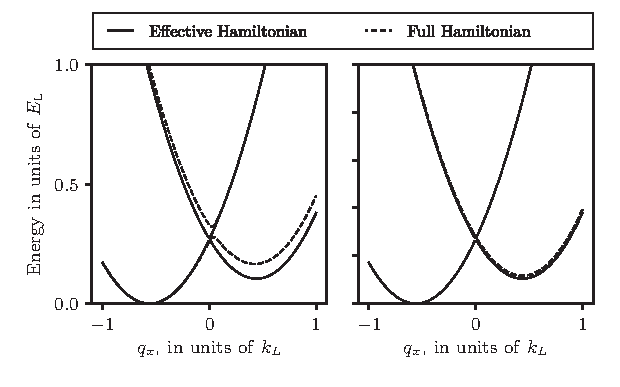
\includegraphics[]{Figures/Chapter8/floquet_effects_legend.pdf}
\caption[Effect of neighboring Floquet manifolds on Rashba dispersion]{Solid lines: Dispersion relation from the effective Floquet Hamiltonian from Equation~\ref{Eq:Rashba_atoms} as a function of $q_x$ for $\Omega_{i,j}=\unit[1.5]{\El}$ and $\delta_i=0$. Dashed lines: Dispersion relation computed for the full Floquet Hamiltonian. We considered $\omega_{zx}=2\omega_{xy}$ and $\omega_{zy}=3\omega_{xy}$ in both cases so the separation between Floquet manifolds is $\omega_{xy}$. In the left panel $\omega_{xy}=\unit[83.24]{kHz}$ as in our experiments and in the right panel $\omega_{xy}=\unit[416.2]{kHz}$. As the spacing between Floquet manifolds becomes larger, the dispersion from the effective and full Hamiltonians become closer.}
\label{fig:floquet_effects}
\end{center}
\end{figure*}

\subsubsection{Lifetime}
There was a lot of concern when we first started setting up to do this experiments about the lifetime of the system due to spontaneous emission being to short. This was in part one of the reasons why we pursued the topology direction rather than trying to measure a fragile many-body phase. The measured spontaneous emission limited lifetime of our system was $\unit[320(17)]{ms}$. However it was reduced to $\unit[40(2)]{ms}$ when we Raman couple the $\xyz$ states, which we attribute to technical noise in the relative phase between the RF dressing field and the Raman laser fields, which has caused considerable consternation in ongoing experiments.  All the experiments reported here were short compared to this timescale so this decreased lifetime was not an issue but it is a limitation that needs to be addressed for future experiments. Figure~\ref{fig:raman_lifetime} shows measurements of the lifetimes of Raman dressed atoms in both $\ket{m_f}$ and $\xyz$ states. We obtained the lifetime by fitting decaying exponentials to the integrated OD from TOF images of thermal atoms where the Raman was turned on in $\unit[1]{ms}$ and held on for up to $\unit[50]{\mu s}$\footnote{How long we could hold on the Raman was limited by the RF antenna heating up.}. 

\begin{figure*}[htb]
\begin{center}
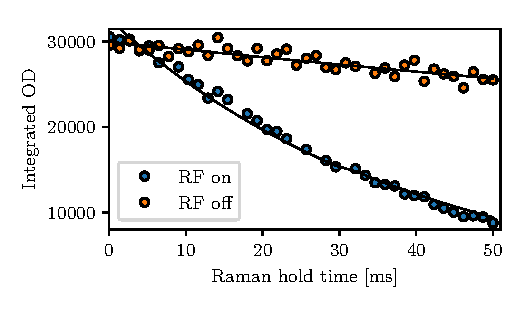
\includegraphics[]{Figures/Chapter8/raman_lifetime.pdf}
\caption[Lifetime of Raman dressed states]{Lifetime of Raman dressed states. We Raman dressed atoms in the $\ket{m_f}$ and $\xyz$ states. The orange markers correspond to atoms initially prepared in $\ket{m_f=-1}$ (no high power RF involved) and the blue markers correspond to atoms $\xyz$ (three averaged traces). The lifetime of doubly dressed states is significantly reduced as compared to the lifetime of the Raman dressed $\ket{m_f}$ states, indicating that of resonant scattering of photons is not our only loss mechanism.}
\label{fig:raman_lifetime}
\end{center}
\end{figure*}

\subsection{Measuring quasimomentum distributions}
Each pair of Raman lasers coupled states $\ket{i, \k}\rightarrow \ket{j, \k+\k_{i,j}}$ where $\ket{i}$ and $\ket{j}$ denote the initial and final $\xyz$ states, $\k$ is the initial momentum and $\k_{i,j}=\k_i-\k_j$ is the two-photon Raman recoil momentum. Dressed states with quasimomentum $\q$ are comprised of three bare states $\ket{j,\k}$ with momentum $\k=\q-\k_j$. The eigenstates of our Rashba SOC Hamiltonian take the form
\begin{equation}
	\ket{\Psi_n(\q)}=\sum_{j\in xyz}\sqrt{a_{n,j}(\q)}e^{i\phi_{n,j}(\q)}\ket{j,\k=\q-\k_{j}},	
	\label{Eq:Raman_wavefunction}
\end{equation}
where the quasimomentum $\q$ is a good quantum number and the amplitudes are parametrized by $a_{n,j}(\q)$ and $\phi_{n,j}(\q)$. We leveraged the wide momentum distribution of a non-condensed ensemble ($T\approx\unit[180]{nK}$ and $T/T_c\approx 1.1$) to sample a wide range of momentum states simultaneously. By starting separately in each of the $\xyz$ states we sampled the range of quasimomentum states shown in Figure~\ref{fig:quasimomentum_map}b, where the momentum distributions of an initial state $\ket{j,\k}$ is shifted from $\q=0$ by the corresponding Raman wave vector $\k_{j}$. 
%
\begin{figure*}[t]
\begin{center}
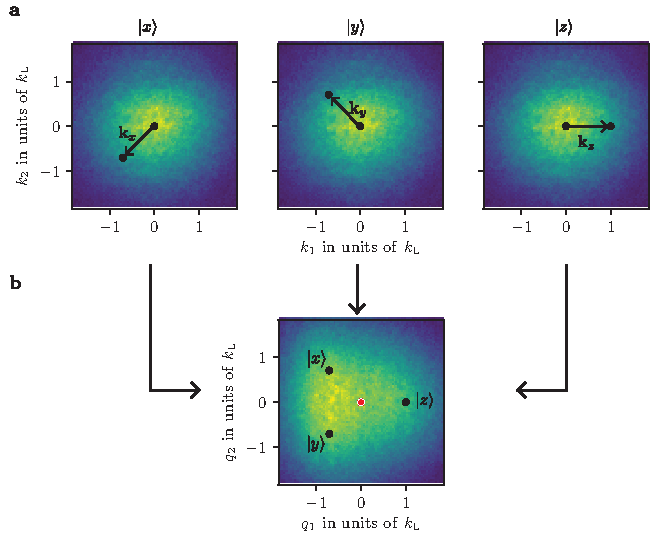
\includegraphics[]{Figures/Chapter8/quasimomentum_map.pdf}
\caption[Mapping momentum into quasimomentum]{Mapping momentum into quasimomentum: {\bf a} We used non-condensed atoms with a broad momentum distribution ($T\approx\unit[180]{nK}$ and $T/T_c\approx 1.1$). {\bf b} Atoms in $\ket{j,\k}$ are mapped to Raman dressed states with quasimomentum $\q=\k+\k_j$. The black dots in the bottom panel represent the location of $\k=0$ for each of the $\xyz$ states and the red dot corresponds to $\q=0$. We performed our experiments starting separately in each of the $\xyz$ states, which allowed us to sample a larger range of quasimomentum states.}
\label{fig:quasimomentum_map}
\end{center}
\end{figure*}

Our measurement protocol consisted of abruptly removing the confining potential and the Raman lasers, initiating a $\unit[21]{ms}$ TOF. During this TOF we adiabatically transformed each of the $\xyz$ states back to a corresponding $\ket{m_F}$ state following the same procedure described in Chapter~\ref{sec:xyz_state_preparation} and spatially separated them using a Stern-Gerlach gradient. Finally we used resonant absorption imaging to measure the resulting density distributions.

The FWHM of the cloud after TOF is about $\unit[700]{\mu m}$ which is much larger than the size of the in-situ cloud $\sim\unit[50]{\mu m}$ and therefore the spatial density distribution of the TOF images represents momentum distribution of the atoms.  For the $\unit[7.4]{\mu m}$ pixel size of our camera and the $3.283$ magnification of our imaging system, the momentum resolution of our images was $\unit[0.018]{\kl}$ and the momentum distributions after TOF had a FWHM of $\sim\unit[2.2]{\kl}$. 

\subsubsection{Correcting shears from gradients}
\begin{figure*}[t]
\begin{center}
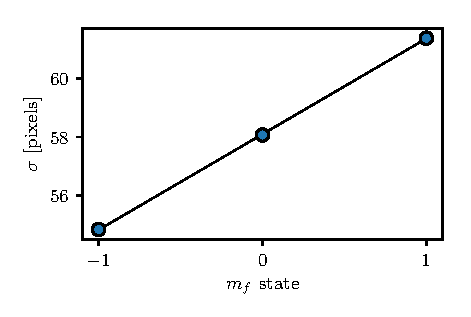
\includegraphics[]{Figures/Chapter8/sg_shear.pdf}
\caption{We measured the standard deviation of the momentum distribution along the axis perpendicular to the SG for 10 shots on each $m_f$ state. From the slope of the linear fit we obtain a shearing parameter $\alpha\approx\pm0.067$ for $m_f=\pm 1$.}
\label{fig:sg_shear}
\end{center}
\end{figure*}

The SG field had a non-zero curvature which caused a compression (or expansion) of the $m_f=-1\ (+1)$ cloud in the direction perpendicular to the SG direction. The projections of a given momentum state $\k$ along the SG axis and perpendicular to it were transformed as $k_{\parallel}\rightarrow k_{\parallel}$ and $k_{\perp}\rightarrow (1+\alpha)k_{\perp}$, where $\alpha=0$ for $m_f=0$ and $\mathrm{sign}(\alpha)=\pm 1$ for $m_f=\pm 1$. Since all our measurements were momentum dependent we had to take special care to quantify and correct this effect on the TOF images. 

We used two different methods to quantify these shears. First we prepared thermal atoms in all three of the $m_f$ states and fit 2D Gaussians rotated by the angle of the SG displacement; $63.8$ degrees for our images. Figure~\ref{fig:sg_shear} shows the standard deviation extracted from the Gaussian fits along the axis perpendicular to the SG deviation as a function of $m_f$ state. We performed a liner fit of $\sigma$ and found that the $m_f=\pm$ states are expanded/contracted by about $\pm 6.7\%$. 

Alternatively we performed the Ramsey interferometer described in Section~\ref{sec:Ramsey} but coupling only 2 states, either $\ket{z}\leftrightarrow\ket{x}$ or $\ket{x}\leftrightarrow\ket{y}$ (mapped to $\ket{-1}\leftrightarrow\ket{0}$ and $\ket{0}\leftrightarrow\ket{+1}$ after TOF). We looked at the oscillation frequencies on each pixel and fit them to Equation~\ref{eq:ramsey_freq} for fixed value of the recoil momentum $\k_{i,j}$ and with a free shear parameter that modifies $\q$. Using this method we extracted a shearing of the order of $7\%$, in good agreement with the Gaussian fitting method.

The transformed momentum coordinates were described by a function $g(\k)=\k^{\mathrm{(shear)}}$ and our observed data $(y_i^{(\mathrm{shear})},\k^{(\mathrm{shear})})$ was the OD in the sheared coordinate system at the $i$th pixel of the CCD sensor. The OD in the unsheared coordinate were estimated using 
%
\begin{equation}
	y_j = \frac{\sum_i\exp[-(g(\k_j)-\k_i^{\mathrm{(shear)}})^2/2\sigma^2]y_i^{\mathrm{(shear)}}}{\sum_i\exp[-(g(\k_j)-\k_i^{\mathrm{(shear)}})^2/2\sigma^2]},
\end{equation}
%
where we used $\sigma$ as the spacing between points in the unsheared coordinate sytem. Prior to any data analysis we applied this transformation to all of our images, where we used different values of $\alpha$ that define $g(\k)$ for each of the $m_f$ states.

\note{TODO: Need to understand origin of this...}
%%%%%%%%%%%%%%%%%%%%%%%%%%%%%%%%%%%%%%%%%%%%%%%%%%%%%%%%%%%%%%%%%%
%
% Results I: Fourier spectroscopy
%
%%%%%%%%%%%%%%%%%%%%%%%%%%%%%%%%%%%%%%%%%%%%%%%%%%%%%%%%%%%%%%%%%

\section{Fourier spectroscopy of the Rashba dispersion}

\begin{figure*}[htb]
\begin{center}
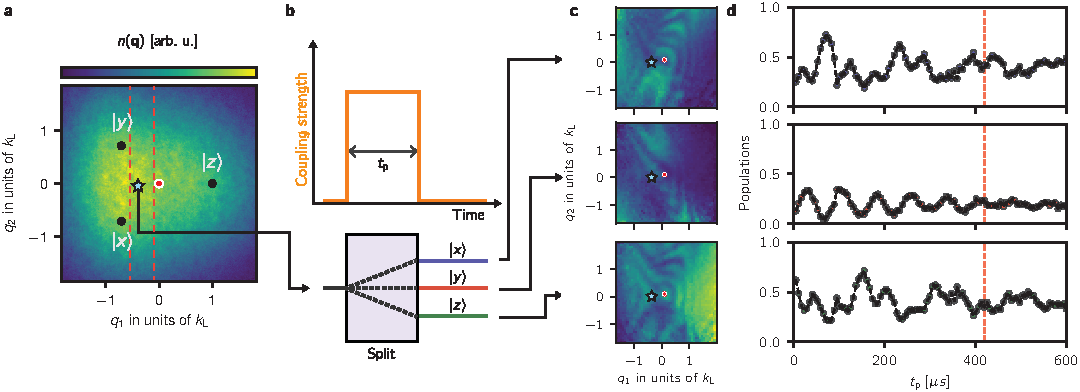
\includegraphics[width=\textwidth]{Figures/Chapter8/fig2.pdf}
\caption{{\bfseries a} Fourier spectroscopy protocol. We applied the Raman lasers for a variable time $t_{\mathrm{p}}$: a Rabi-type atomic interferometer analogous to a three-port beam splitter. {\bfseries b} Probabilities as a function of quasimomentum for a fixed Raman pulse time $t_{\rm p}=\unit[420]{\mu s}$ {\bfseries c} Dynamics of the final populations of the $\xyz$ states with quasimomentum $(q_1, q_2)=\unit[(-0.55,-0.18)]{k_{\rm L}}$ (blue star in panels {\bfseries b}) after initializing the system in the $\ket{z}$ state. }
\label{fig:fourier_spectroscopy}
\end{center}
\end{figure*}

We directly measured the 2D dispersion relation using Fourier transform spectroscopy\cite{valdes-curiel_fourier_2017} (see Chapter~\ref{ch:Fourier_spectroscopy}). In this technique we considered the evolution of an initial state $\ket{i,\mathbf{k}}$ suddenly subjected to the Raman coupling lasers. This atomic Rabi-type interferometer is analogous to the three-port beam-splitter depicted in Figure~\ref{fig:fourier_spectroscopy}b. During a pulse time $t_{\mathrm{p}}$ we followed the dynamics of the populations in the $\xyz$ states which evolved with oscillatory components proportional to $\sum_{j\neq n} a_{n,j}(\q)\cos([E_n(\q)-E_{j}(\q)]t_{\mathrm{p}}\,/\hbar)$, with frequencies determined by the eigenenergy differences $E_n-E_j$. Figure~\ref{fig:fourier_spectroscopy}c shows the momentum dependent populations for a fixed pulse time $t_{\mathrm{p}}$ and Figure~\ref{fig:fourier_spectroscopy}d shows representative final populations as a function of $t_{\mathrm{p}}$ for a fixed quasimomentum state. We Fourier transformed the populations with respect to $t_p$ and for a given quasimomentum state for a total of 9 state, all of them with the same $\q$ accounting for each of the three initial $\xyz$ states that was then split into 3 states. Figure~\ref{fig:fourier_grid} shows the PSD computed for each of the 9 states for planes of constant $q_1$. The amplitude of the oscillatory components depends on the overlap integral between the initial state and the Raman dressed states as was discussed in Chapter~\ref{ch:Fourier_spectroscopy} so sampling all these states gave us access to a wider range of measurable frequencies. The spectral maps in Figure~\ref{fig:fourier_spectroscopy_bands}b were produced by averaging the PSDs from the 9 different states using $\bar{n}$, the mean population in $t_{\rm p}$, as a weight:
%
\begin{equation}
	\mathrm{PSD}^{(\rm{mean})}(\q) = \frac{\sum_{i,j}\mathrm{PSD}_{i,j}(\q)\bar{n}_{i,j}(\q)}{\sum_{i,j}\bar{n}_i,j(\q)},
\end{equation}
%
where the indices $i,j$ represent the different states of the grid shown in Figure~\ref{fig:fourier_grid}. The extrema in the spectral maps are the energy differences $E_n-E_j$ in the engineered dispersion (Figure~\ref{fig:fourier_spectroscopy}a). The combined maps show the presence of a single Dirac point in the Rashba subspace, evidenced by the gap closing near $\q=0$ and the photon-like lower branch. The dashed curves correspond to the energy differences computed for our system using the dispersions shown in Figure~\ref{fig:fourier_spectroscopy_bands}a, and are in clear agreement with our experiment. %This measurement directly confirms the expected set of energies, including the existence of a two-state subspace approximately described by the Rashba Hamiltonian. 
\begin{figure*}[htb]
\begin{center}
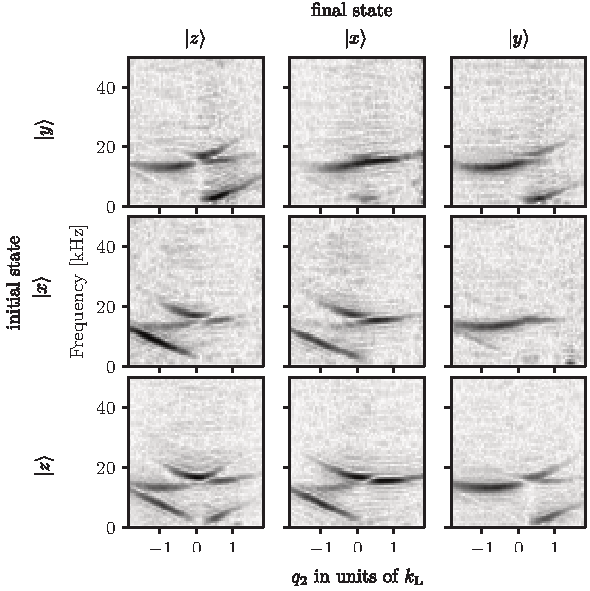
\includegraphics[]{Figures/Chapter8/fourier_grid.pdf}
\caption{Something}
\label{fig:fourier_grid}
\end{center}
\end{figure*}

\begin{figure}[htb]
\begin{center}
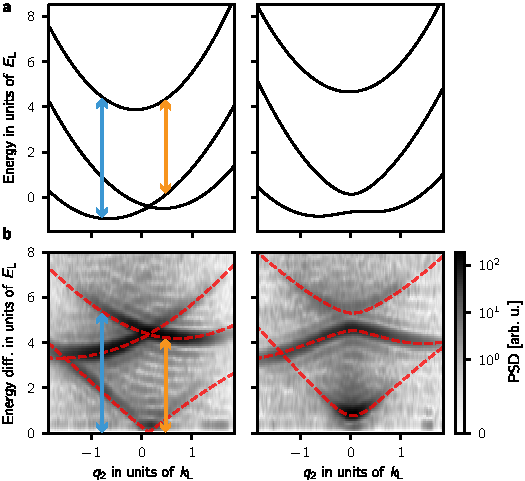
\includegraphics[]{Figures/Chapter8/fig3.pdf}
\caption{{\bfseries a} Predicted dispersion relation as a function of $q_2$ for fixed $q_1=-0.09 \,k_{\rm L}$ (left) and $0.65\,k_{\rm L}$ (right), computed for the experiment parameters. The energy differences between the branches enclosing the vertical arrows appear as peaks in the spectral maps below. {\bfseries b} Power spectral density (PSD) for the same parameters as above which we obtained by Fourier transforming the populations in the $\xyz$ states with respect to $t_{\mathrm{p}}$. The dashed lines correspond to the energy differences computed using the dispersion curves on the top panel.}
\label{fig:fourier_spectroscopy_bands}
\end{center}
\end{figure}


%%%%%%%%%%%%%%%%%%%%%%%%%%%%%%%%%%%%%%%%%%%%%%%%%%%%%%%%%%%%%%%%%%
%
% Results II: Measurement of Chern number
%
%%%%%%%%%%%%%%%%%%%%%%%%%%%%%%%%%%%%%%%%%%%%%%%%%%%%%%%%%%%%%%%%%%
%
\section{Quantum state tomography with Ramsey interferometer}
\label{sec:Ramsey}

The Fourier spectroscopy measurement confirmed our quantum engineering of the Rashba Hamiltonian. However, the energies shed no light on the topology of the different branches of the dispersion, which instead requires knowledge of the eigenstates. The Berry curvature present in the definition of the Chern number (Equation~\ref{eq:chern_number}) can be derived from the Berry's connection $\mathbf{A}_n(\q)=i\bra{\Psi_n(\q)}\mathbf{\nabla}_q\ket{\Psi_n(\q)}$, which as discussed in Chapter~\ref{ch:Topology} behaves much like a vector potential in classical electromagnetism. The Berry curvature $\mathbf{\Omega}_n(\q)=\mathbf{\nabla}_q\times\mathbf{A}(\q)$ is the associated magnetic field and the flux through any surface is the line integral of $\mathbf{A(\q)}$ along its boundary, after neglecting the contributions of Dirac strings which we will discuss later. Using the expression for the Raman dressed eigenstates from Equation~\ref{Eq:Raman_wavefunction} we obtain
%
\begin{equation}
 \mathbf A_n(\q)= -\!\!\!\!\!\!\sum_{j \in\{x, y, z\}}  a_{n,j}(\q)  \nabla_q \phi_{n,j}(\q),
\label{Eq:Berry_connection1}
\end{equation}
%
which depends on both the phase and amplitude of the wave function.  We obtained $a_{n,j}(\q)$ and $\phi_{n,j}(\q)$ using a three-arm time-domain Ramsey interferometer, implementing a variant of quantum state tomography\cite{flaschner_experimental_2016,godfrin_generalized_2018}. The use of a multi-path interferometer allowed us to transduce information about phases into state populations, which we readily obtained from absorption images. 
%
\begin{figure*}[htb]
\begin{center}
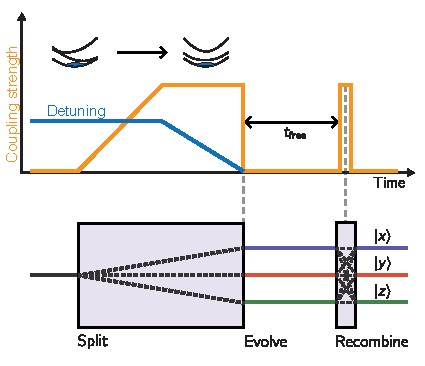
\includegraphics[]{Figures/Chapter8/fig4a.pdf}
\caption{Experimental protocol for three-arm Ramsey interferometer (not to scale). (Top) We started with atoms in state $\ket{z,y,\q_i=\k+\mathbf{k}_j}$ and with detuning $\delta_y=\pm \unit[5]{E_{\rm L}}$ and $\delta_z=\pm\unit[5]{E_{\rm L}}$. We ramped the Raman lasers on in $750 \us$ and then ramped the detuning to nominally zero. We let the system evolve in the dark for times between $5 \,\us$ and $400\,\us$, followed by a $\unit[25]{us}$ Raman pulse. (Bottom) The implemented experimental protocol was equivalent to a three-arm interferometer that split an initial state into three final states with amplitudes related to the initial wave function phases.}
\label{fig:Ramsey_ramps}
\end{center}
\end{figure*}

Figure~\ref{fig:Ramsey_ramps} shows our experimental protocol which I will describe in detail in more detail in the following section. We adiabatically mapped an initial $\ket{j, \k}$ state into a corresponding eigenstate $\ket{n,\q=\k+\k_j}$, either in the topologically trivial highest dispersion branch ($n=3$) or in the topological ground branch ($n=1$) by dynamically tailoring both the Raman coupling strength and detuning. We suddenly turned off the Raman coupling, thereby allowing the three bare state components of the Rashba eigenstates to undergo free evolution for a time $t_{\mathrm{free}}$, constituting the three arms of our time-domain interferometer. Finally we applied a three-port beam splitter using a brief Raman `recombination' pulse to interfere the three arms. 

\subsection{Wave function evolution in Ramsey interferometer}

{\bf Rashba dressed state preparation:} We started with $\xyz$ states at different coupling strength $\Omega_{\rm RF}/\pi 2\pm \unit[20]{kHz}$, such that the energies of the $\ket{z}$ and $\ket{y}$ states were shifted by about $\pm \unit[18.8]{kHz}$. We used the same Raman frequencies as described earlier and therefore the change in the $\xyz$ state eigenenergies corresponded to non-zero $\delta_z$ and $\delta_y$ in Equation~\ref{Eq:Rashba_atoms}. We chose the detuning such that the initial state had a large overlap with either the $n=1$ or the $n=3$ eigenstates of Equation~\ref{Eq:Rashba_atoms}. We then ramped on the Raman coupling in $\unit[750]{\mu s}$, adiabatically mapping the $\ket{z}$ and $\ket{y}$ states into the $n=1$ or $n=3$ eigenstates. Because our only experimental knob for dynamically changing the detuning was $\Omega_{\rm{RF}}$ we could not control $\delta_x$ so when we initialized the system in $\ket{x}$ the the final dressed state always corresponded to the $n=2$ branch. After turning on the Raman we ramped $\Omega_{\rm RF}$ to its final value in $\unit[1]{ms}$, effectively ramping $\delta_z$ and $\delta_y$ close to zero. This detuning ramp had the additional effect of moving the location Dirac point through the atoms, thereby creating a trajectory where the state preparation was not adiabatic. This trajectory depended on the sign of the detuning ramp and combining data from different initial states allowed us to exclude the Dirac point trajectories. Near the final location of the Dirac point the state preparation can not be adiabatic regardless of the initial state or detuning used for the ground state preparation. At the end of this stage, the state of the system was described by the eigenstates in Equation~\ref{Eq:Raman_wavefunction}.

{\bf Free evolution:} We suddenly turned off the Raman coupling, thereby projecting the Raman dressed states back into the $\xyz$ basis. Each of the $\xyz$ state represents a different branch of the interferometer and they acquire phases that are proportional to $t_{\rm{free}}$
%
\begin{equation}
	\ket{\Psi_n(\q)}\rightarrow \sum_{j\in xyz}\sqrt{a_{n,j}(\q)}e^{i\phi_{n,j}(\q)}e^{-iE_j(\q)t_{\rm{free}}/\hbar}\ket{j,\k=\q-\k_{j}},
\end{equation}
%
where $E_j(\q)=\hbar^2\q^2/2m$ is the free particle energy. One subtle difference between our interferometer and other types of interferometers is that in our case the phase that we are interested in measuring is imprinted when the state is split. The dynamical phases $E_j(\q)t_{\rm{free}}/\hbar$ acquired in the different interferometer arms does not contribute to our knowledge of the Rashba eigenstates as they describe the evolution of the system in the absence of Raman dressing. 

{\bf Recombination pulse:} We applied a $\unit[25]{us}$ Raman pulse that acted as a second beam splitter in our interferometer sequence. The wave function after the pulse is
%
\begin{equation}
	\ket{\Psi(\q)}= \sum_{j,j'\in xyz}\sqrt{a_{n,j}(\q)}e^{i(\phi_{n,j}(\q)-E_j(\q)t_{\rm{free}}/\hbar)} U_{j,j'}(\q)\ket{j,\k=\q-\k_{j}},
\end{equation}
%
where $U_{j,j'}(\q)=\vert U_{j,j'}(\q)\vert \exp(i\phi_{j,j'}^{\rm{(pulse})}(\q))$ is the matrix element of the unitary transformation $\exp(i\hat H_{\rm R}(\q) t_{\rm{pulse}})$ associated to the Raman pulse. At the end of this procedure, the population in a final state $\ket{l, \q}$ is
\begin{equation}
P_l(\q,t)=\sum_{i\neq j} \vert U_{l,i}\vert \vert U_{j,l}\vert \sqrt{a_{n,i} a_{n,j}}\cos(\omega_{i,j}(\q) t+\phi_{n,i}(\q) - \phi_{n,j}(\q)+\phi_{l,i,j}^{(\rm{pulse})}(\q)),
\label{Eq:Ramsey_evolution}
\end{equation}
which directly reads out the phase differences, independent of the output port $l$. Here $\phi_{l,i,j}^{(\rm{pulse})}=\phi_{j,l}^{\rm{(pulse})}-\phi_{l,i}^{\rm{(pulse})}$ is a smoothly varying phase imprinted by the recombination pulse and is independent of $\q$ in the limit of short, strong pulses. The angular frequencies
%
\begin{equation}
	\omega_{i,j}(\q)=\hbar \q \cdot \k_{i,j}/m + \delta_{i,j}
	\label{eq:ramsey_freq}
\end{equation}
%
result from the known free particle kinetic energy, the recoil momenta and detuning $\delta_{i,j}$ from the tripod resonance condition. Figure~\ref{fig:Ramsey_ramps}b shows the momentum-dependent populations in each output port at fixed $t_{\rm free}=\unit[160]{\mu s}$ and Figure~\ref{fig:Ramsey_ramps}c shows the populations as a function of $t_{\mathrm{free}}$ for a representative quasimomentum state $(q_1, q_2)=(0.55,-0.92)\,k_{\rm L}$.  

\begin{figure*}[htb]
\begin{center}
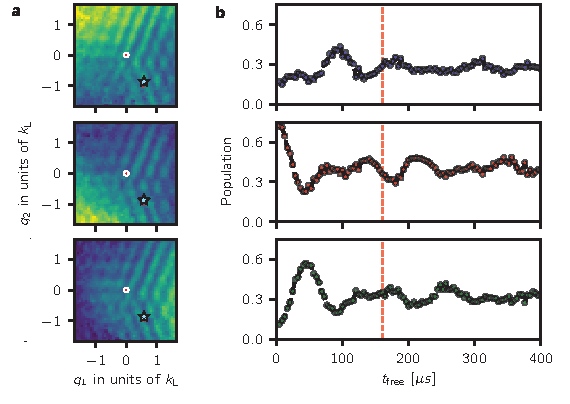
\includegraphics[]{Figures/Chapter8/fig4bc.pdf}
\caption{{\bfseries a} Probabilities as a function of quasimomentum for the three output ports of the interferometer at $t_{\rm free}=\unit[160]{\mu s}$ {\bfseries b} Probabilities as a function of free evolution time $t_{\mathrm{free}}$ for an input state with quasimomentum $(q_1, q_2)=(0.55,-0.92)\,k_{\rm L}$ indicated by the blue star on {\bfseries a} and in the topological ground branch ($n=1$)}
\label{fig:Ramsey_fringes}
\end{center}
\end{figure*}

We obtained the relative phases $\Delta\phi_{n,i,j,l}=\phi_{n,i}(\q) - \phi_{n,j}(\q)+\phi_{l,i,j}^{\rm{(pulse)}}(\q)$ from Equation~\ref{Eq:Ramsey_evolution} by fitting the measured populations to the sum of three cosines with the known free particle frequencies but unknown amplitudes and phases. 

\subsection{Recombimation pulse effects}
The last term $\Delta\phi_{n,i,j,l}$ arises from the recombination pulse in the interferometer. It corresponds to a smooth $\q$-dependent variation along the Raman recoil axis $\k_{i,j}$ with an additional $\q$-independent offset that depends on the state index $l$. The presence of this extra term does change the measured topological index (see Appendix~\ref{app:Ramsey_phases}).

When combining the phases all measurements got rid of the $l$ dependent offset by shifting $\Delta\phi_{n,i,j,l}$ by a constant number such that there was a maximal overlap for all phases. This shift was constant in $\q$ and had no effect on the topological index. 

\subsection{Combining phases from all states}

The largest value of $t_{\mathrm{free}}$ in the experiment limits how well we can resolve the phases of low frequencies $\omega_{ij}(\q)$ near $q=0$ as well as when two different frequencies $\omega_{ij}(\q)$ and $\omega_{i'j'}(\q)$ are close to each other, as can be seen in the high noise present in the phase-maps near $q=0$ as well as in lines where the fit frequencies become nearly degenerate. This limitation is reflected in the large variation in the Berry phase depicted in the shaded region of Figure~\ref{fig:Ramsey_phases}c near $q=0$.

Finally, we averaged all the phase differences obtained from the fits, weighted by the inverse of the uncertainties obtained from the fitting procedure. For the topological branch data we excluded the regions away from $\q=0$ where the Dirac point was moved from the average. Finally we chose a gauge such that $\phi_1(\q)=0$ and used this to convert phase dif

\begin{figure*}[htb]
\begin{center}
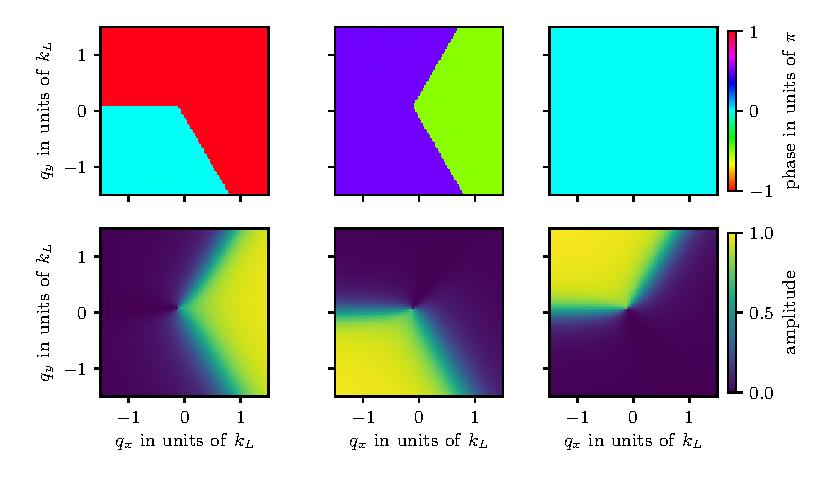
\includegraphics[]{Figures/Chapter8/topological_eigenvecs.pdf}
\caption{{\bfseries a} Probabilities as a function of quasimomentum for the three output ports of the interferometer at $t_{\rm free}=\unit[160]{\mu s}$ {\bfseries b} Probabilities as a function of free evolution time $t_{\mathrm{free}}$ for an input state with quasimomentum $(q_1, q_2)=(0.55,-0.92)\,k_{\rm L}$ indicated by the blue star on {\bfseries a} and in the topological ground branch ($n=1$)}
\label{fig:topological_eigenvecs}
\end{center}
\end{figure*}

\begin{figure*}[htb]
\begin{center}
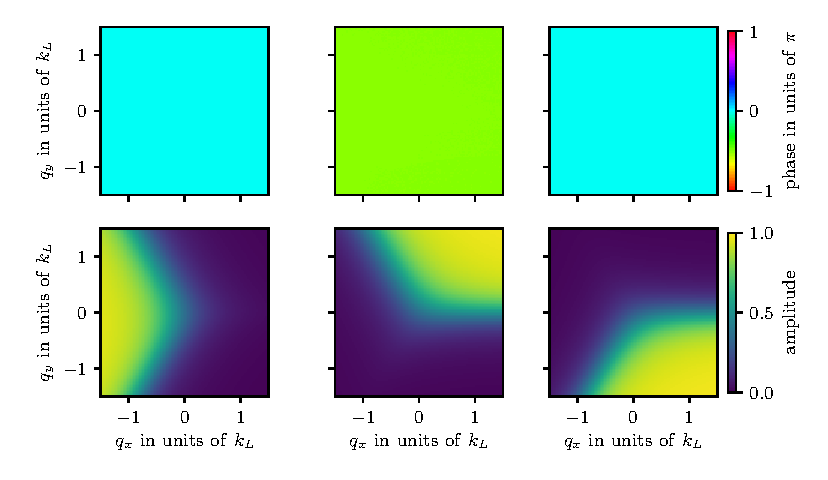
\includegraphics[]{Figures/Chapter8/nontopological_eigenvecs.pdf}
\caption{{\bfseries a} Probabilities as a function of quasimomentum for the three output ports of the interferometer at $t_{\rm free}=\unit[160]{\mu s}$ {\bfseries b} Probabilities as a function of free evolution time $t_{\mathrm{free}}$ for an input state with quasimomentum $(q_1, q_2)=(0.55,-0.92)\,k_{\rm L}$ indicated by the blue star on {\bfseries a} and in the topological ground branch ($n=1$)}
\label{fig:nontopological_eigenvecs}
\end{center}
\end{figure*}


\subsection{Measuring the topological index}

Figure~\ref{fig:Ramsey_phases}a shows typical phase-maps for both the non-topological and topological branches. In the non-topological phase-maps the momentum dependence of the recombination pulse $\phi_{l,i,j}^{p}(\q)$ causes a smooth variation of the phases along the Raman recoil axes that does not affect the evaluation topological index of our system. To recover the phases $\phi_{n,j}$ of the full spinor wave function from the fits, we made the gauge choice described in the Methods.

We recovered the phases $\phi_{n,j}$ of the full spinor wave function from the relative phases obtained from the fits by choosing a particular gauge such that $\phi_{n,0}=0$. We then used the values of $a_{n,i}$ obtained from measuring the populations in the $\xyz$ states at $t_{\mathrm{free}}=0$ in combination with the phases of the wave function to compute the Berry connection\cite{fukui_chern_2005}. Figure~\ref{fig:Ramsey_phases}b shows the three phase differences as a function of polar angle for a loop of radius $q\approx 0.77\,k_{\rm L}$ for both the topological and non-topological branches. In addition to the smooth variations induced by the recombination which are present in both columns, the phases of the topological branch have two $\pi$ valued jumps that lead to non-zero Berry phases when the Berry connection is integrated along a closed loop in momentum space. Figure~\ref{fig:Ramsey_phases}c shows the integrated Berry phase as a function of loop radius. For loops with $q>0.4\,k_{\rm L}$ we obtain an integrated Berry phase that suggests an asymptotic Chern number of $\Phi_{\rm B}/2\pi=0.01(1)$ for the non-topological branch and $\Phi_{\rm B}/2\pi=0.5(5)$ for the topological branch. However, Berry's phase measurements including ours includes the (potential) contribution of any Dirac strings traversing the integration area. In our system, these are possible at the Dirac point $^*$, and each contributes $\pm2\pi$ to $\Phi_{\rm B}$ as was discussed in Chapter~\ref{sec:Dirac_string}. Even with this $2\pi$ ambiguity we are able to associated a half-integer Chern number with the topological branch, which is possible only for a topological dispersion branch in the continuum. 
\begin{figure}[htb]
\begin{center}
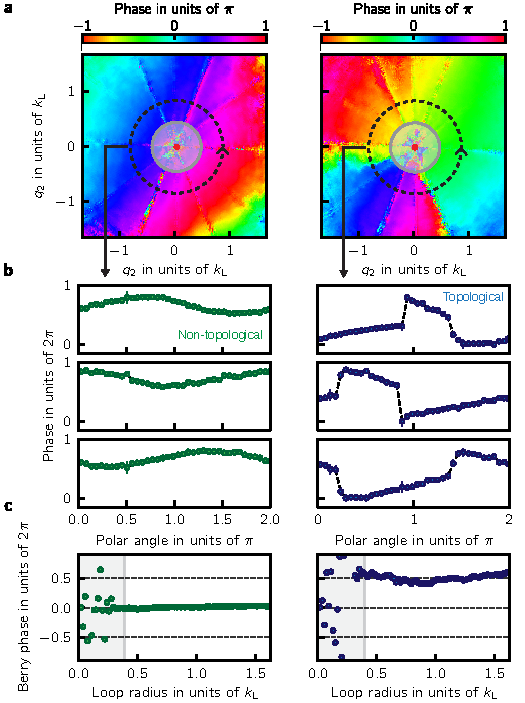
\includegraphics[]{Figures/Chapter8/fig5.pdf}
\caption{Topological invariants from quantum state tomography, for the non-topological branch ($n = 3$, left) and the topological branch ($n = 1$, right). {\bfseries a} Phase differences as a function of quasimomentum from the the $z\rightarrow x$ transition {\bfseries b} Phase differences as a function of polar angle for a loop radius $\unit[0.77]{\kl}$ from the $z\rightarrow x$ (top), $x\rightarrow y$ (middle) and $y\rightarrow z$ (bottom) transitions. The phases associated to the topological branch are characterized by two $\pi$ valued discontinuities. Each row of phases was shifted by a constant value so that the three rows of phases share the same vertical axis. All phases shown here were binned and averaged using the fit uncertainties as weights. {\bfseries c} Inferred Chern number as a function of loop radius. For loops with $q>0.4\,k_{\rm L}$ we obtained an integrated Berry phase and asymptotic Chern number of $\Phi_{\rm B}/2\pi=0.01(1)$ for the non-topological branch and $\Phi_{\rm B}/2\pi=0.5(5)$ for the topological branch.}
\label{fig:Ramsey_phases}
\end{center}
\end{figure}

\section{Conclusion}

In conventional lattices --- for example graphene, or the topological Haldane model --- it is well established that Dirac points each contribute a Berry's phase of $\Phi_{\rm B} /2\pi =\pm 1/2$\cite{duca_aharonov-bohm_2015}, but crystalline materials conspire for these to appear in pairs\cite{nielsen_adler-bell-jackiw_1983}, always delivering integer Chern numbers. In contrast, our continuum system contains a single Dirac point, resulting in a non-integer Chern number. This leads to intriguing questions about edge states at interfaces with non-integer Chern numbers with non-integer Chern number differences. Initial studies in the context of electromagnetic waveguides\cite{silveirinha_chern_2015 } and atmospheric waves\cite{delplace_topological_2017} have applied Chern invariants and the bulk-edge correspondence to continuous media. 

While the true Rashba Hamiltonian features a ring of degenerate eigenstates, our implementation including the quadratic and cubic Dresselhaus-like SOC lifts this macroscopic degeneracy giving three nearly degenerate minima\cite{campbell_realistic_2011}. Already these three minima could allow the study of rich ground state physics in many body systems of bosons, for example the formation of fragmented BECs\cite{stanescu_spin-orbit_2008} when the system does not condense into a single-particle state. Furthermore, the use of additional spin states or larger Raman couplings can partially restore this degeneracy allowing the possible realization of fractional Hall like states\cite{sedrakyan_statistical_2015}. 

% \note{Modify words} Our present work clearly shows new non-integer values for topological invariants, but leaves open the “bulk-boundary” connection, which links quantized transport to interfaces between systems with different topological invariants.


%%%%%%%%%%%%%%%%%%%%%%%%%%%%%%%%%%%%%%%%%%%%%%%%%%%%%%%%%%%%%%%%%
%
%Methods
%
%%%%%%%%%%%%%%%%%%%%%%%%%%%%%%%%%%%%%%%%%%%%%%%%%%%%%%%%%%%%%%%%%%



%%%%%%%%%%%%%%%%%%%%%%%%%%%%%%%%%%%%%%%%%%%%%%%%%%%%%%%%%%%%%
%
%Graveyard
%
%%%%%%%%%%%%%%%%%%%%%%%%%%%%%%%%%%%%%%%%%%%%%%%%%%%%%%%%%%%%%
% \textit{Fiber bundles} A manifold is a topological space which looks locally like $R^n$ , but not necessarily so globally. A fibre bundle is, so to speak, a topological space which looks locally like a direct
% product of two topological spaces. 

% systems with Rashba-type~\cite{bychkov_oscillatory_1984} spin-orbit coupling represents can be

% Often, systems with SOC will have multiply degenerate single particle eigenstates with topological character: this suggests that strongly correlated phases will exist in the presence of interactions for both bosonic and fermionic systems

% which can be understood as non-Abelian gauge potential, is an important ingredient for realizing $\mathds{Z}_2$ topological insulators and the quantum spin Hall effect~\cite{kane_$z_2$_2005,hasan_colloquium:_2010} 

% There has been a lot of interest in the community to engineer non-abelian gauge potentials in ultracold atomic systems~\cite{ruseckas_non-abelian_2005}. In particular Rashba-type spin-orbit coupling 

% The SO interaction plays an essential role in topological insulators, which have been predicted and experimentally discovered in two-dimensional (2D) and 3D materials (1, 2), and topological superconductors (3, 4), which host exotic zero-energy states called Majorana fermions (5) and still necessitate rigorous experimental verification. For topological insulators, the strong SO interaction leads to band inversion, which drives topological phase transitions in such systems. In superconductors, triplet p-wave pairing may occur when SO coupling is present and results in topologically nontrivial superconductivity under proper conditions (6).

% SOC is pervasive in material systems. In some cases it leads to parasitic effects such as reduced spin coherence times [197], while in other contexts, like topological insulators, it is essential [74, 198]. Topological insulators—non-interacting fermionic systems—represent a first realization of time- reversal (TR) invariant systems with topological order [74]. In analogy with the progression from the TR-violating single- particle IQHE to the interaction driven fractional quantum Hall effects (FQHEs), the next important step is realizing strongly interacting cousins to the topological insulators, of which topological superconductors are a first example [199, 200]. Ultracold atoms are an ideal platform to study strongly interacting SOC systems, both with bosonic [165] and fermionic atoms [50].

% Abelian gauge potentials (7, 8), can enable the study of a broader range of nontrivial quantum states such as topological insulators driven by 2D and 3D SO interactions (1, 2). Furthermore, a 2D SO interaction is the minimal requirement to reach a gapped topological superfluid phase through a conventional s-wave superfluid state (22, 23).

% The topology of Bloch bands defines integers that serve to both classify crystalline materials and precisely specify properties, such as conductivity, that are independent of small changes to lattice parameters\cite{hasan_colloquium:_2010}. Topologically non-trivial materials first found application in metrology with the definition of the von Klitzing constant as a standard of resistance, which is now applied in the realization of the kilogram\cite{newell_codata_2018}. Today, topological systems have found applications in the engineering of low loss optical waveguides\cite{ozawa_topological_2019} and present a promising path to quantum computation\cite{nayak_non-abelian_2008}.

% Both the Euler characteristic and the Chern number are integer valued, but the Euler characteristic depends only on the manifold $\mathcal{M}$ and its intrinsic curvature, whilst the Chern number depends both on a manifold (the BZ) and an additional vector field defined on $\mathcal{M}$ (the Berry curvature). 


% As discussed in Chapter~\ref{ch:Topology}, a central tenet in topological matter is the existence of integer valued `invariants' that are independent of small changes to parameters. 


% For an arbitrary closed 2-manifold $\mathcal{M}$ and a suitable choice of vector field (i.e., a two-form) $\mathbf{\Omega}$ the surface integral
% %
% \begin{equation}
% 	\frac{1}{2\pi}\int_{BZ}\mathbf \Omega\cdot d\mathbf S
% 	\label{Eq:topology}
% \end{equation}
% %


% In contrast, when $\mathcal{M}$ is a torus describing a two-dimensional Brillouin zone (BZ) and $\mathbf{\Omega}$ is the Berry curvature that characterizes the underlying quantum states, Equation~\ref{Eq:topology} instead gives the Chern number. 


% There has been considerable interest in engineering non-Abelian gauge potentials in ultracold atomic systems~\cite{wilczek_appearance_1984,ruseckas_non-abelian_2005}. In particular, Rashba-type~\cite{bychkov_oscillatory_1984}, an example of a non-Abelian gauge potential, has multiply degenerate single particle eigenstates which could open the possibility of studying strongly correlated phases in the presence of interactions for systems of both fermions and bosons~\cite{stanescu_spin-orbit_2008,sedrakyan_composite_2012,hu_probing_2011}. 

% However, in order to observe meaningful many-body physics it is necessary to have a long lived system and even though 2D SOC has been previously realized in ultracold $^{40}$K\cite{huang_experimental_2016} the experiments were limited by the collisional relaxation lifetime due to the coupling of atoms in different hyperfine manifolds. These concerns motivated a new proposal~\cite{campbell_rashba_2016} to engineer Rashba SOC within the ground hyperfine manifold of alkali atoms using the RF dressed $\xyz$ states discussed in Chapter~\ref{ch:clock_states} and Raman transitions. 

% Even though this new proposal offered many advantages compared to previous experiments, we were still feeling very pessimistic about the lifetime of our system mostly because of spontaneous emission from the Raman lasers. Rather than trying to measure a fragile many-body phase we decided to instead shift our focus into topology as the Rashba Hamiltonian has a topologically non-trivial dispersion relation. Unlike conventional materials, there is no underlying crystalline structure leading to Chern numbers that can take unconventional half-integer values. 

%  for both a topologically trivial and non-trivial configuration, where it respectively takes the value of zero or a half integer
